\subsection{Central Limit Theorem}


Under certain conditions, the normal distribution can be used to approximate probabilities for linear combinations of random variables having a non-normal distribution. This follows from the Central Limit Theorem (C.L.T.). 

The normal distribution is commonly used because it tends to approximate the distribution of sums of random variables.


\begin{theorem}[\textbf{Central Limit Theorem}]
    \phantom{}  \\
    If $X_1, X_2, \ldots, X_n$ are \textbf{independent} random variables all having the \textbf{same distribution},
    with mean $\mu$ and variance $\sigma^2$, then as $n \to \infty$, the cumulative distribution
    function (c.d.f.) of the random variable
    \[\frac{\dis \sum_{i=1}^n X_i - n\mu}{\sigma \sqrt{n}} = \frac{S_n - n\mu}{\sigma \sqrt{n}}\]
    approaches the $N(0, 1)$ cumulative distribution function. Similarly, the cumulative distribution
    function of 
    \[\frac{\overline{X} - \mu}{\frac{\sigma}{\sqrt{n}}}\]
    approaches the $N(0, 1)$ cumulative distribution function.
\end{theorem}

\begin{remark}
    For large $n$, we have
    \begin{itemize}
        \item $S_n = \displaystyle \sum_{i=1}^{n} X_i \sim \text{N}(n\mu, n\sigma^2)$.
        \item $\overline{X} = \frac{1}{n} \displaystyle \sum_{i=1}^{n} X_i \sim \text{N}(\mu, \frac{\sigma^2}{n})$.
    \end{itemize}
    If $X_i$'s themselves have normal distributions, then $S_n$ and $\overline{X}$ have \textbf{exactly} normal distributions $\forall n$. Otherwise, $S_n$ and $\overline{X}$ have \textbf{approximately} normal distributions.
\end{remark}

\pagebreak

General idea of the C.L.T. is that it takes any distribution and makes it normal.
\begin{figure}[htbp]
    \center
    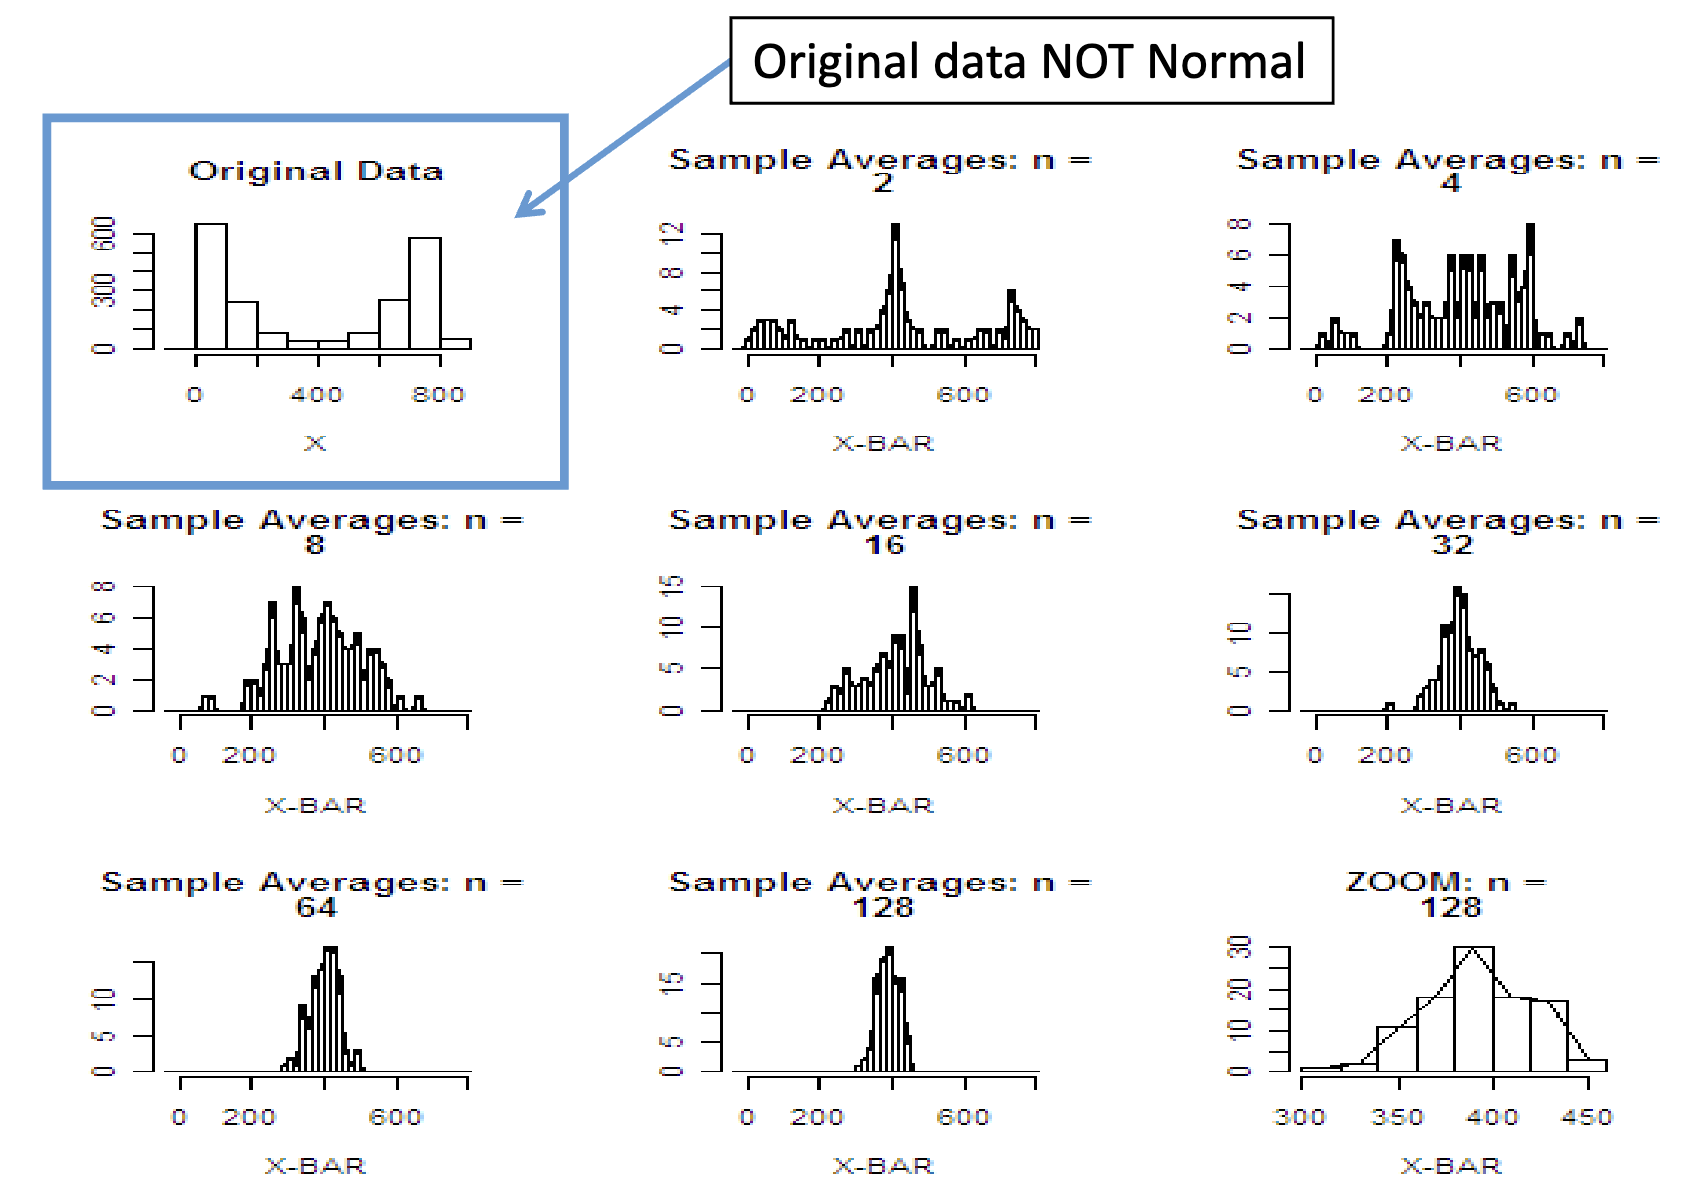
\includegraphics[scale=0.5]{img/CLT-ex.png}
    \caption{Visualizing the idea of CLT.}
\end{figure}

\begin{example}
    Suppose fires reported to a fire station satisfy the conditions for a Poisson process, with a mean of 1 fire every 4 hours. Find the probability the $500^{\text{th}}$ fire of the year is reported on the $84^{\text{th}}$ day of the year.

\end{example}

\begin{theorem}[\textbf{Normal Approximation to Poisson}]
    \phantom{}  \\
    Suppose $X \sim Poisson(\mu)$. Then the cumulative distribution function of the standarized
    random variable
    \[Z = \frac{X - \mu}{\sqrt{\mu}}\]
    approaches that of a standard Normal random variable as $\mu \to \infty$.
\end{theorem}

\begin{theorem}[\textbf{Normal Approximation to Binomial}]
    \phantom{}  \\
    Suppose $X \sim Binomial(n, p)$. Then for large $n$, the random variable
    \[W = \frac{X - np}{\sqrt{np(1 - p)}}\]
    has approximately a $N(0, 1)$ distribution.
\end{theorem}


\subsection{Moment Generating Functions}

\begin{definition}[\textbf{Moment Generating Functions}]
    \phantom{}\\
    Consider a discrete random variable $X$ with probability function $f(x)$. The moment generating function (m.g.f.) of $X$ is defined as \vspace{-3mm}
    \[
        M(t) = \expect{e^{tX}} = \displaystyle \sum_{\text{all $x$}} e^{tx} f(x).
    \]
    We will assume that the moment generating function is defined and finite for values of $t$ in an interval around 0 (i.e. for some $a > 0$, $\displaystyle \sum_{x} e^{tx} f(x) < \infty \; \forall t \in [-a,a]$).
\end{definition}

\begin{theorem}
    \phantom{}\\
    Suppose the random variable $X$ has moment generating function $M(t)$ defined $\forall t \in [-a,a]$ for some $a > 0$. Then \vspace{-3mm}
    \[
        \expect{X^k} = 
    \]
\end{theorem}



\subsection{Motivariate Moment Generating Functions}









\newpage